% paper=a4paper (default),letterpaper,a5paper,b5paper,executivepaper,legalpaper
% font=
% fontsize=10pt, 11pt, 12pt (10pt por defecto)
% documentclass=article,report,book,letter,"ieeetran"
% draft=draft (no carga imagenes, pero indica lugares)
% columns=onecolumn(default), twocolumn
% margenes=oneside,twoside
\documentclass[
    a4paper,
    12pt
]{article}

\usepackage{times}
%\usepackage[options]{paquete}
%\usepackage[spanish]{babel}
%\usepackage[utf8]{inputenc}
%\usepackage[T1]{fontenc}
%\usepackage{graphicx}
%\usepackage{amsmath}

\title{Titulo del trabajo}
\date{\today}
\author{Autor o autores}

\usepackage{lipsum}

\begin{document}
	\maketitle
	\begin{abstract}
		\lipsum[1-2]
	\end{abstract}
	%\clearpage

    \section{Viñetas y enumeraciones}

	\begin{itemize}
		\item Un contenido extremadamente largo para que sirva de ejemplo
		\item Dos
		\item Tres
		\begin{itemize}
			\item Tres Uno
			\item Tres Dos
		\end{itemize}
	\end{itemize}
%
	\begin{enumerate}
		\item Uno
		\item Dos
		\begin{enumerate}
			\item Anidado
		\end{enumerate}
		\begin{itemize}
			\item Viñeta
			\item Otra viñeta
		\end{itemize}
		\item Cuatro
	\end{enumerate}

	\begin{description}
		\item[Etiqueta] Descripcion
		\item[RDBMS] Sistema de administracion de bases de datos
	\end{description}

    \begin{center}
        \lipsum[1]
    \end{center}

    \begin{quote}
        \lipsum[1]
    \end{quote}

    \begin{quotation}
        \lipsum[1]
    \end{quotation}

	%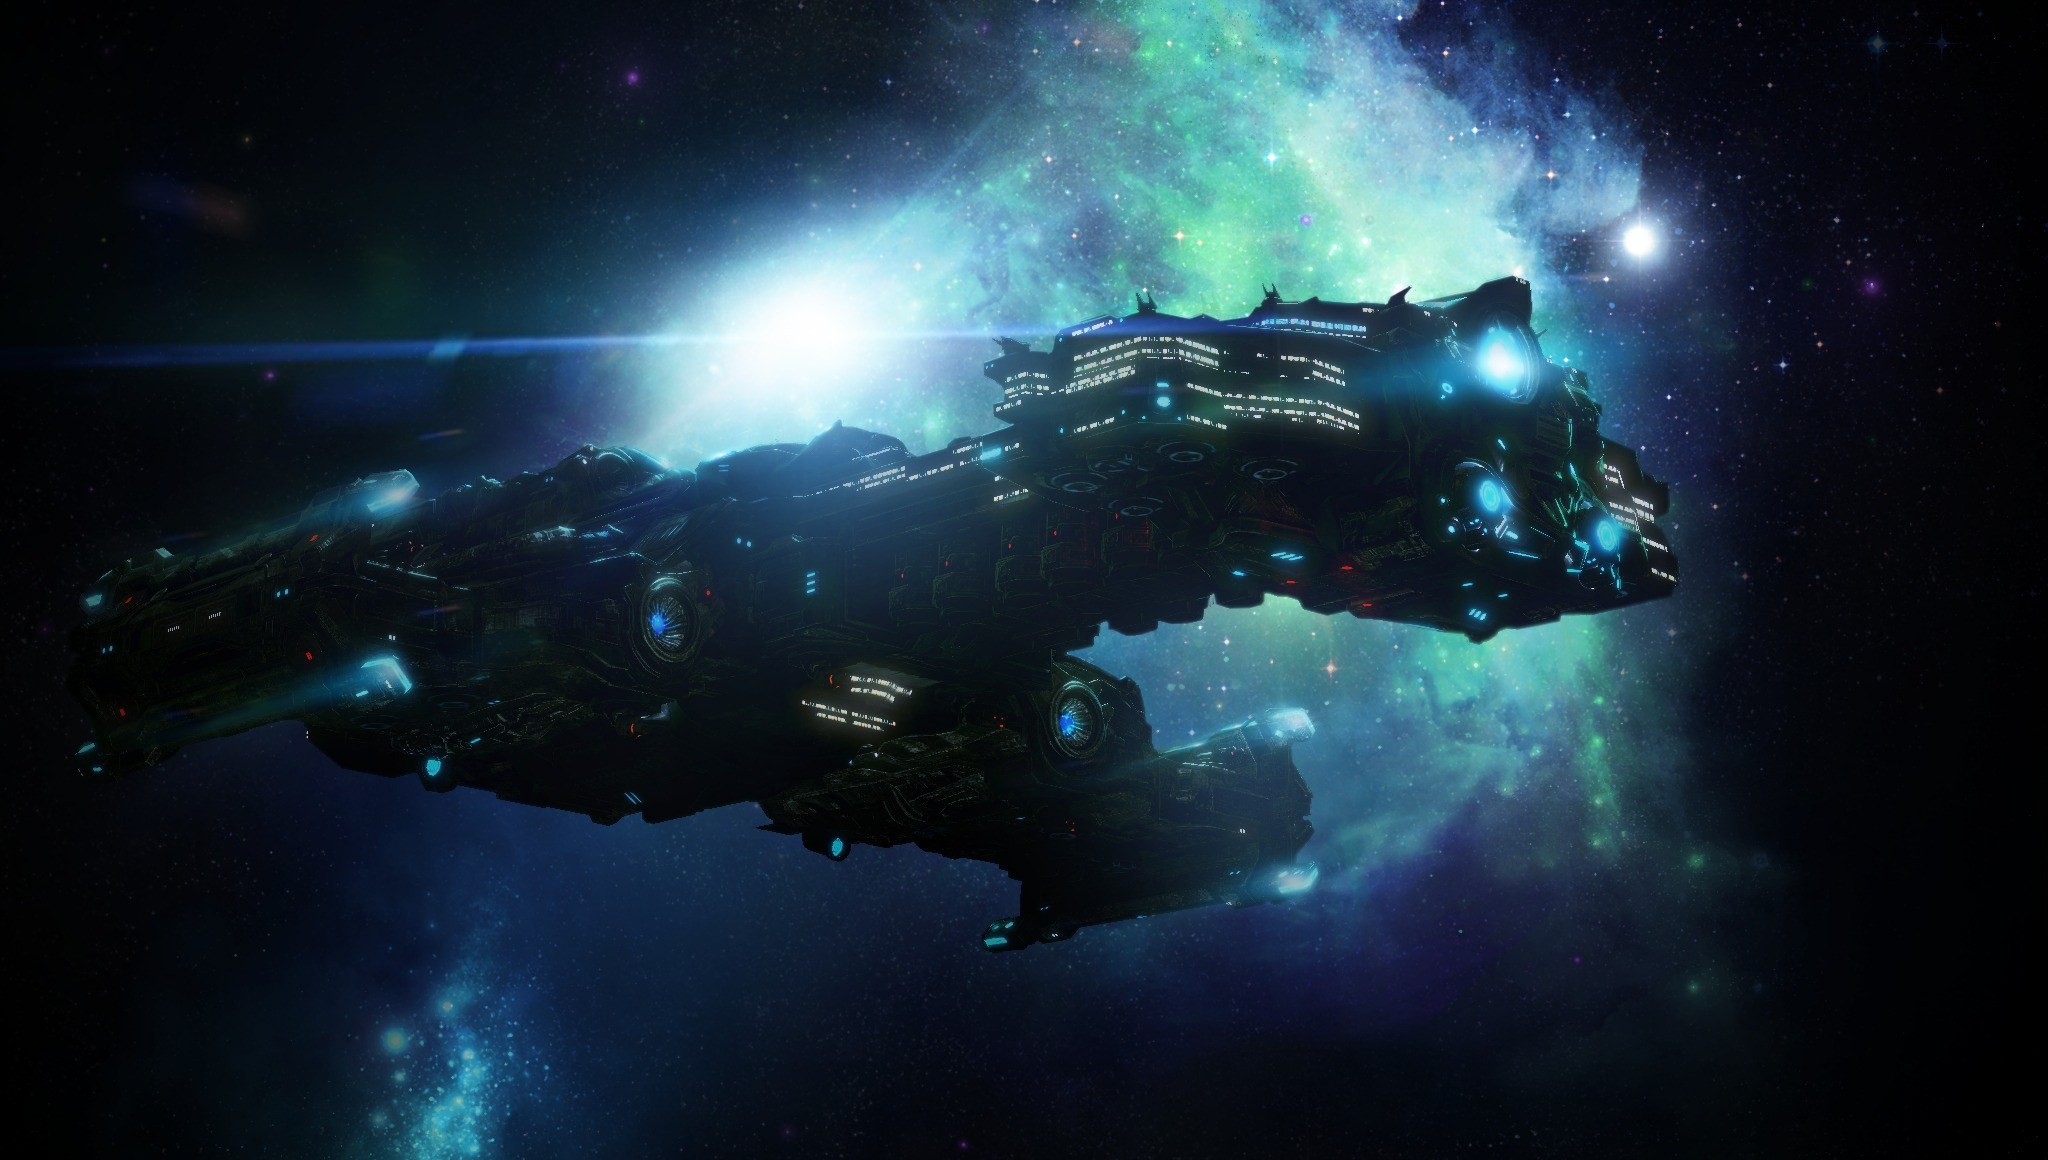
\includegraphics[scale=0.1]{ship1}
	%
\includegraphics[width=250px]{tech1}
	
\end{document}